% This is a document written to introduce students in MATH 2300-04 at FSU to LaTeX and Overleaf.  Any other students are free to use this as well.

% All of this stuff with '%' in front is a comment and ignored by the compiler.
%
% The lines before the "\begin{document}" line is called the preamble.
% This is where you load particular packages you need.
% Until you are more experienced, or the program says you are missing packages, it is safe to ignore it.
%
%----------------------------------

\documentclass[12pt]{article}
\usepackage[margin=1in]{geometry}% Change the margins here if you wish.
\setlength{\parindent}{0pt} % This is the set the indent length for new paragraphs, change if you want.
\setlength{\parskip}{5pt} % This sets the distance between paragraphs, which will be used anytime you have a blank line in your LaTeX code.
\pagenumbering{gobble}% This means the page will not be numbered. You can comment it out if you like page numbers.


%These packages allow the most of the common "mathly things"
\usepackage{amsmath,amsthm,amssymb}

\usepackage{mathtools,pgfplots,graphicx}
%This package allows you to add graphs or any other images.
\usepackage{graphicx}
\usepackage[utf8]{inputenc}


%These are the packages I usually use and needed for this document. There are bajillions of others to do nearly antyhing you want.
\usepackage{color}
\usepackage{enumerate}
\usepackage{multicol}

\newcommand{\pn}[1]{\left( #1 \right)}

\newtheorem{theorem}{Theorem}

%------------------------------------------
% The stuff you want to edit starts here.
%------------------------------------------
\begin{document}

\title{Matrix Eggs} % You should make this the title of your project.
\author{Tommy Schneider, Cassidy Le, Joe Nunez} % Replace this with your name.
% \date{} I have this commented out so that the program will use whatever today's date is.  You can specify a particular date (or use this for other info if you need) in the {} or leave the {} empty for no date (or other extra info) to appear in the title

\maketitle

\section{Basics of Principle Component Analysis}
\section{Matrix Eggs}
\subsection{Basic Examples}
\begin{enumerate}
	\item Solid Color
	\item Noise
\end{enumerate}
\section{Visualization Method 1: Heat Maps}
One simple way of making sense of the distance matrix between two sets of matrix eggs is by plotting them as a heat map.
\subsection{Anomaly Detection in Spot the Difference Photos}
One application
Take, for example, the following two $386\times 350$ images:
\begin{center}
	\begin{tabular}{c c}
		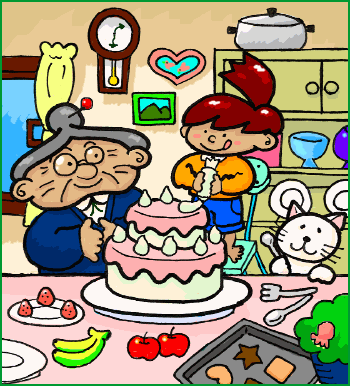
\includegraphics[scale=0.5]{spot_left.png} & 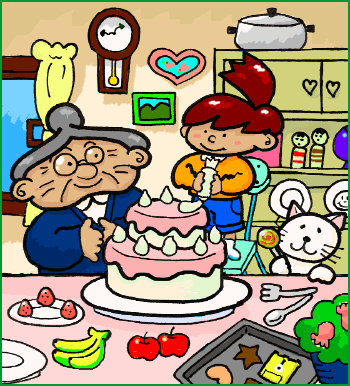
\includegraphics[scale=0.5]{spot_right.png} \\
	\end{tabular}
\end{center}
\begin{center}
	\begin{tabular}{c c}
		
\includegraphics[scale=0.5]{spot_100_100.png} & 
\includegraphics[scale=0.5]{spot_50_50.png} \\
		$100 \times 100$  & $50 \times 50$ \\
		
\includegraphics[scale=0.5]{spot_25_25.png} & 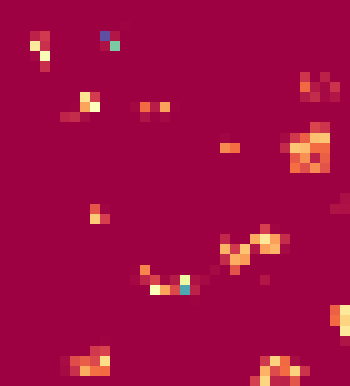
\includegraphics[scale=0.5]{spot_10_10.png} \\
		$25 \times 25$  & $10 \times 10$ \\
		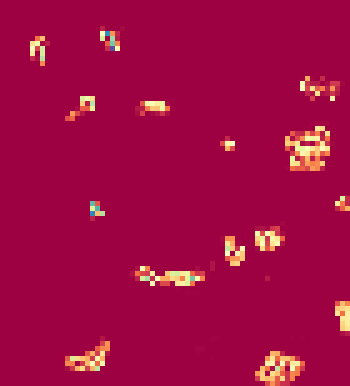
\includegraphics[scale=0.5]{spot_5_5.png} & 
\includegraphics[scale=0.5]{spot_2_2.png} \\
		$5 \times 5$  & $2 \times 2$ \\
	\end{tabular}
\end{center}


\subsection{Videos}

\section{Anomaly Detection in Brain Tumor Images}

\end{document}